\textbf{Исходный текст:} \\
    The XSL attack is not an attack. It is a dream

\textbf{Ключ:} \\
    OY8Y?Fa??FHc<4bRJ3?AFLQWFXUFPUIF

\textbf{Зашифрованный текст:} \\
    678c20e1607b836fc27446e815ac306c3c559a9bc8c6d1b5d 257f6a9893e9a6c70f36f9cb83a23123ca9b5f779c99cae

Результаты работы программы представлены на рисунках~\ref{ris:encode-test-5}-\ref{ris:decode-test-5}.

\vspace{\baselineskip}
\begin{figure}[H]
\center{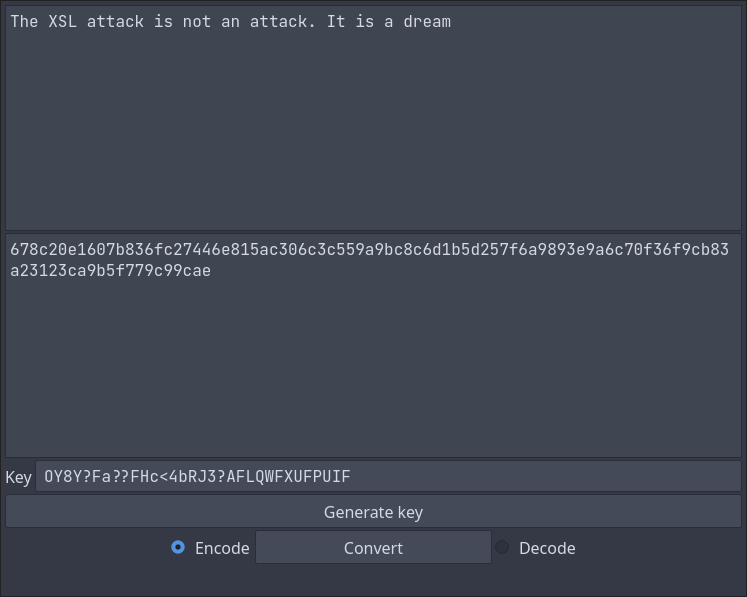
\includegraphics[width=0.8\linewidth]{figures/encode-test-5}}
    \caption{Шифрование}
\label{ris:encode-test-5}
\end{figure}

\vspace{\baselineskip}
\begin{figure}[H]
\center{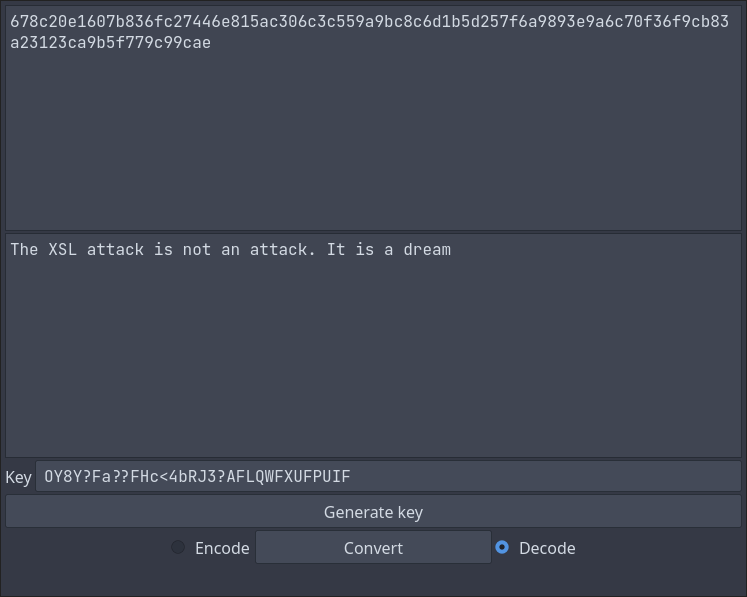
\includegraphics[width=0.8\linewidth]{figures/decode-test-5}}
    \caption{Расшифрование}
\label{ris:decode-test-5}
\end{figure}
